\section{Задание 2}

Организовать показ слайд шоу из этих же картинок, чтобы каждая следующая картинка показывалась не автоматически, а при нажатии кнопки.

При нажатии на кнопку ``[Следующая картинка]'':

\begin{center}
  
\includegraphics[width=10cm]{img/Exercise_02/01.png}
  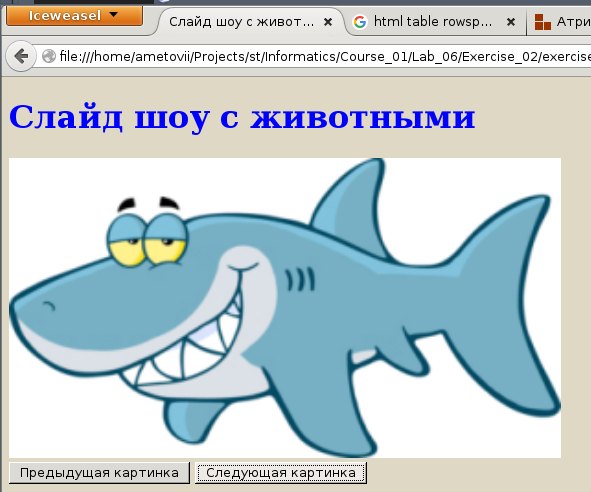
\includegraphics[width=10cm]{img/Exercise_02/02.png}
  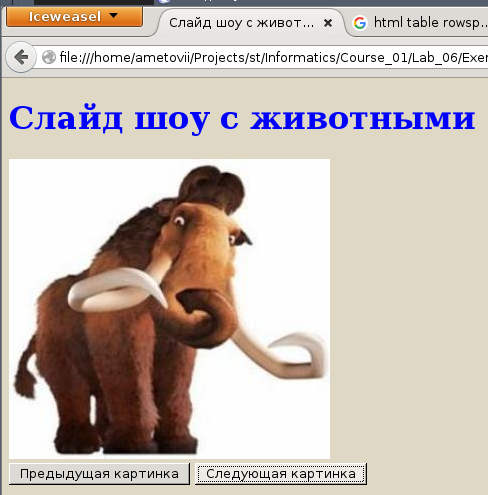
\includegraphics[width=10cm]{img/Exercise_02/03.png}
\end{center}

При нажатии на кнопку ``[Предыдущая картинка]'':

\begin{center}
  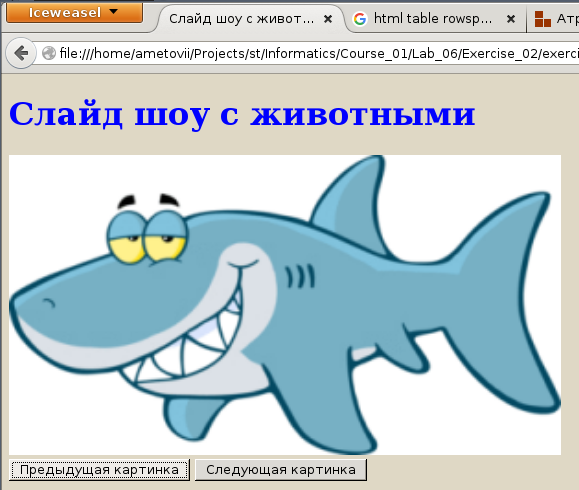
\includegraphics[width=10cm]{img/Exercise_02/04.png}
\end{center}

Исходный код \verb|exercise_02.html|:


\begin{verbatim}
<!doctype html>
<html>
  <head>
    <title>Слайд шоу с животными</title>
    <meta charset='utf-8' />
     <style type="text/css">
      body {background-color:#dfd8c5; color:#0000ff;}
      img {width:274; height:233}
     </style>
     <script>
       currentImage=0;
       var lowerBound=0;
       var upperBound=2;
       
       var imageSources=["Images/begemot.jpg",
			 "Images/shark.png",
			 "Images/mamont.jpg"];
       function nextImage(){
	   if (currentImage==upperBound) currentImage=lowerBound;
	   else currentImage=currentImage+1;
	   var someImage=document.getElementById('pic');
	   someImage.src=imageSources[currentImage];
       }

       function previousImage(){
	   if (currentImage==lowerBound) currentImage=upperBound;
	   else currentImage=currentImage-1;
	   var someImage=document.getElementById('pic');
	   someImage.src=imageSources[currentImage];
       }
     </script>
     </head>
  <body>
    <h1>Слайд шоу с животными</h1>
    <img name="pic" id='pic' src="Images/begemot.jpg" /><br>
    <input type="button" value="Предыдущая картинка"
	   onClick="previousImage()" />
    <input type="button" value="Следующая картинка"
	   onClick="nextImage()" />
  </body>
</html>
\end{verbatim}
